\section{Arbeitsschritte}
 
\subsection{Design des instrumentierten Schüttguts}
\subsubsection{Kriterien für das instrumentierte Schüttgut}

Allgemeine Anforderungen an das instrumentierte Schüttgut:

\begin{itemize}
	\item Möglichst klein, maximale Größe der Module \textsuperscript{1\\)}
	\item Aufnehmen/Speichern von Bewegungsdaten
	\item Übertragung von Daten an einen PC
	\item Betrieben durch interne Batterie
	\item Optional: Cachen von Daten, bis diese ausgelesen werden 
\end{itemize}

\textsuperscript{1\\)} Das instrumentierte Schüttgut soll in eine Kapsel eines Kinder-Überraschungseis passen. Dadurch wird die maximale Größe des Schüttguts festgelegt. Die Wahl der Ü-Ei-Kapsel als Hülle für das Schüttgut eignet sich dahingehend gut, dass es einerseits den Mikrocontroller schützt, andererseits sehr einfach zu beschaffen ist und kein Behältnis aufwendig produziert werden muss (zum Beispiel mittels 3D-Druck).

\begin{figure}[ht]
	\centering
	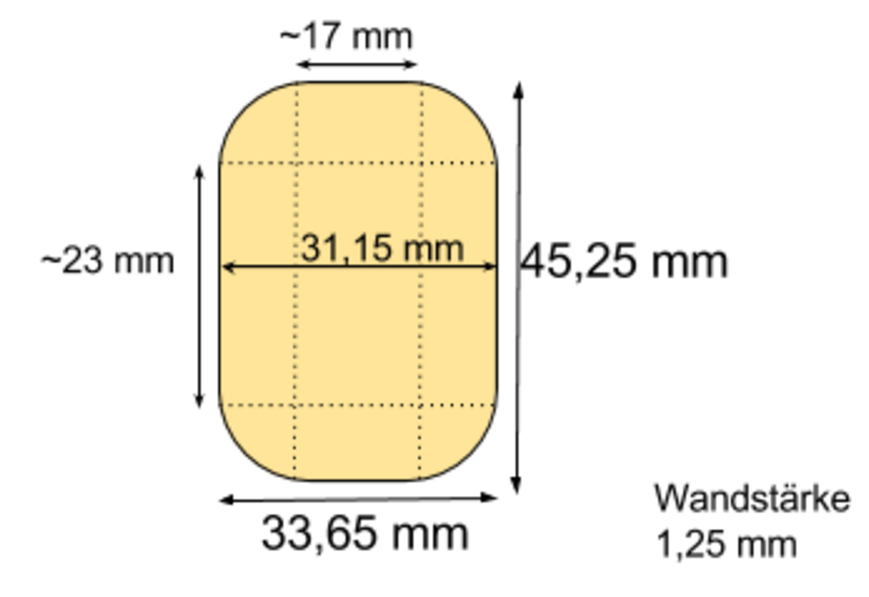
\includegraphics[width=0.5\textwidth]{images/k3-ueei.PNG}
	\caption {Maße der Kapsel aus einem Kinder Überraschungsei}
	\label{fig:k3}
\end{figure}

Die Beschaffung der Bauteile sollte zudem möglichst einfach sein. Von Vorteil ist, wenn alle Bauteile von einem deutschen Händler bezogen werden könnten, um einerseits nur einen einzelnen Liefervorgang zu haben und andrerseits eine geringere Lieferzeit (anstatt international). Auch eine ausreichende Dokumentation der einzelnen Module ist sehr nützlich für eine schnelle Implementierung des Mikrocontroller-Codes. Die einzelnen Module müssen kompatibel zueinander sein.

\subsubsection{Recherche}
Begonnen wurde mit einer Recherche, welche Bauteile es gibt, mit denen sich solch ein instrumentiertes Schüttgut erstellen lässt. Als Hauptplatine wird ein Mikrocontroller benötigt, an dem weitere Bauteile angeschlossen werden können. Es gibt einzelne Sensormodule, die z.B.Orientierung und Beschleunigung in je 3 Achsen gleichzeitig messen können. Ebenso gibt es verschiedene Speicher- und Übertragungsmodule, die Daten auf eine SD-Karte loggen oder per Bluetooth / WLAN / ZigBee weiterleiten können. Ausschlaggebend bei der Wahl der einzelnen Module war zunächst die Größe der einzelnen Bauteile, die selbst die Größe eines Ü-Eis nicht übersteigen dürfen. Nach der Wahl eines passenden Mikrocontrollers müssen auch die Anschlussmöglichkeiten für weitere Module mit beachtet werden.

\textbf{Mikrocontroller}, Gewähltes Bauteil: Adafruit Pro Trinket 3V 12MHz

Der Pro Trinket 3V 12MHz von Adafruit besitzt einen leistungsstarken ATmega328-Chip, der auch auf einigen Arduino-Mikrocontrollern verwendet werden. Er besitzt einen Speicher von 28K und einen RAM von 2K. Vorteile sind bei diesem, dass er jedoch mit 18 GPIOs (General Purpose Input Output) und 2 analogen Anschlüssen weitaus mehr Anschlussmöglichkeiten bietet, als beispielsweise der Arduino Pro Mini. Die Maße des Boards sind  38mm x 18mm x 4mm, sodass die Platine ausreichend Platz in der Kapsel haben sollte. Auf dem Trinket ist ein USB Bootloader vorinstalliert, sodass der Mikrocontroller per USB programmiert werden kann. (Quelle: \url{https://www.adafruit.com/products/2010}, 12.05.2016)

\textbf{Aufnahme von Bewegungsdaten}, Gewähltes Bauteil: Adafruit 9-DOF IMU Breakout - L3GD20H + LSM303

Das Modul L3GD20H kann drei verschiedene Datentypen in jeweils drei Achsen messen: Beschleunigungsdaten, Rotationsdaten und Magnetische Achsen ähnlich zu einem Kompass. Da Beschleunigungs- und Gyroskopdaten gemessen werden sollen, ist ein Bauteil, dass beide Daten zusammen liefern kann, sehr platzeffizient. Die Kommunikation zwischen dem Mikrocontroller und dem Datensensor benutzt das I2C-Protokoll. Das Bauteil hat die Maße 38mm x 23mm und ist damit um 5 Millimeter breiter als der Mikrocontroller Pro Trinket. (Quelle: \url{https://www.adafruit.com/products/1714}, 12.05.2016)

\textbf{Übertragung der Daten}

Zur möglichst unkomplizierten Übertragung von Daten an den PC wird eine drahtlose Verbindung verwendet. Dadurch ergeben sich drei verschiedene mögliche Typen:
\begin{itemize}
	\item ZigBee: Zu Aufwändig, da ein separates Modul für den PC benötigt wird. Hingegen sind fast alle Laptops heute standardmäßig mit WLan und Bluetooth ausgestattet.
	\item WLAN: Die zur Auswahl stehenden Platinen sind entweder deutlich zu groß, oder in ihrer Verwendung zu heikel, da sie extrem empfindlich auf kleinste Spannungsschwankungen reagieren. Zudem ist der Stromverbrauch größer als bei Bluetooth. Da das Schüttgut nur durch eine sehr kleine Batterie betrieben werden kann, ist dies hinderlich.
	\item Bluetooth: Bluetooth ist weit verbreitet und die Module sind klein genug, um sie mit im Ü-Ei unterzubringen.
\end{itemize}

Gewähltes Bauteil: Adafruit Bluefruit LE SPI Friend - Bluetooth Low Energy (BLE)

Gewählt wurde das Adafruit Bluefruit LE SPI Friend, dass durch Bluetooth Low Energy sehr energiearm sein soll. Zur Kommunikation mit dem Mikrocontroller wird das Protokoll SPI benutzt. Mit den Maßen 23mm x 26mm x 5mm ist es dicker als die anderen Bauteile, aufgrund der geringeren Breite sollte sich das Bauteil dennoch in der Rundung des Ü-Eis Platz finden. Das Modul hat außerdem Speicherplatz von 256KB. (Quelle: \url{https://www.adafruit.com/products/2633}, 12.05.2016)

\textbf{Betrieb durch interne Batterie}, Gewählte Bauteile: Adafruit Pro Trinket LiIon/LiPoly Backpack Add-On, Lithium Ion Polymer Battery - 3.7v 150mAh

Um einen universellen Einsatz des instrumentierten Schüttguts zu garantieren, muss es mit einer eigenen Batterie oder einem eigenen Akkumulator betrieben werden. 
Mit dem Adafruit Trinket Lilon Backpack Add-On lässt sich ein Akkumulator an das Pro Trinket anschließen. Das Add-On dient als Ladestation, wenn das Pro Trinket per USB mit einem Rechner verbunden ist. Sobald der USB-Port entfernt wird, schaltet das Modul automatisch in den batteriebetriebenen Modus. Das Modul hat eine Größe von 15mm x 17mm x 7mm. Die relativ große Höhe im Vergleich zu den anderen Modulen kommt durch den Anschluss für den Akkumulator zustande. (Quelle: \url{https://www.adafruit.com/products/2124}, 12.05.2016)

Hinzu kommt eine Lithium Ion Polymer Battery mit 3,7V und 150mAh. Dieser Akku wurde aufgrund der geringen Größe von 19,75mm x 26mm x 3,8mm gewählt. Es gibt auch Modelle mit mehr Kapazität, die aber auch andere Abmessungen besitzen. Zum Teil geht die Länge über 30mm hinaus. Es werden allerdings schon Bauteile über diese Länge verwendet, die in der vertikalen Achse der Kapsel platziert werden müssen. Der Akku sollte daher näher an der Aussenwand positioniert werden, wo die Höhe durch die Abrundung der Kapsel jedoch eingeschränkt wird. (Quelle: \url{https://www.adafruit.com/products/1317}, 12.05.2016)

\textbf{Alternative Überlegungen zum Cachen der Daten}

Da die meisten Mikrocontroller nur sehr wenig eigenen Speicher haben und eine drahtlose Datenverbindung nicht zuverlässig genug ist, müssen die vom Sensor gelesenen Daten auf einem extra hinzugefügten Speicher zwischen gespeichert werden, bis sie vom PC ausgelesen werden können.

Mögliche Bauteile: Adafruit I2C Non-Volatile FRAM Breakout - 256Kbit / 32KByte (Quelle: \url{https://www.adafruit.com/products/1895}, 12.05.2016), Adafruit SPI Non-Volatile FRAM Breakout - 64Kbit / 8KByte (Quelle: \url{https://www.adafruit.com/products/1897}, 12.05.2016) 

Vorerst sind diese Bauteile out of scope, da das Bluetooth Modul über 256 KB Speicher verfügt, die eventuell als Cache bzw. Puffer genutzt werden können.
Mit den gewählten Bauteilen lässt sich der Speicher des Mikrocontrollers von den integrierten 28 KB (schon abzüglich der 4 KB für die Dateien des Bootloaders) auf um 8 bzw. 32  KB erhöhen. 

Die gewählten Bauteile sind alle von der Marke Adafruit. Der Vorteil darin liegt in der Kompatibilität der Bauteile aufgrund der Abstimmung zueinander, sowie in der sehr ausführlichen Dokumentation dieser. 

\textbf{Verwendete Hardware}

\begin{table}[h]
	\centering
	\begin{tabular}{|l|c|}
		\hline
		\textbf{Bauteil} & \textbf{Menge} \\
		\hline
		 Adafruit Pro Trinket 3V 12MHz & 3 \\
		 \hline
		 Adafruit 9-DOF IMU Breakout - L3GD20H + LSM303 & 3 \\
		 \hline
		 Adafruit Bluefruit LE SPI Friend - Bluetooth Low Energy (BLE) & 3 \\
		 \hline
		 Adafruit Pro Trinket LiIon/LiPoly Backpack Add-On & 3 \\
		 \hline
		 Lithium Ion Polymer Battery - 3.7v 100mAh\textsuperscript{*)} & 9 \\
		 \hline		 
	\end{tabular}
		\caption{Bestellte Hardware}
		\label{tab:bestellteHW}
\end{table}

\textsuperscript{*)} Aufgrund von der Nichtverfügbarkeit des gewünschten Akkus bei einem Lieferanten musste ein anderer Akku gewählt werden. Dadurch konnte die Bestellung aber bei nur einem Lieferanten getätigt und eine kurze Lieferzeit erreicht werden.

\begin{table}[h]
	\centering
	\begin{tabular}{|l|c|}
		\hline
		\textbf{Materialien} & \textbf{Menge} \\
		\hline
		Breadboard & 2 \\
		\hline
		Set mit Steckkabeln & 2 \\
		\hline
		Arduino Uno & 1 \\
		\hline	
		Arduino Duemilanove & 1 \\
		\hline	
		Ardunio Feather & 1\\
		\hline
	\end{tabular}
	\caption{Weitere Hilfsmittel stehen zur Verfügung}
	\label{tab:verfuegbareHW}
\end{table}

\subsubsection{Machbarkeitsstudie}

Vor der Bestellung wurden noch einige Machbarkeitsstudien durchgeführt. Neben dem Vergleich gegenüber anderen verfügbaren Modulen wurde ein Größentest durchgeführt und eine Wiring-Skizze angefertigt.

Bei dem Größentest wurden die einzelnen Module Maßstabsgetreu mit Moosgummi nachgebaut. Dadurch konnte getestet werden, wie sich die Module am besten in der Ü-Ei-Kapsel anordnen lassen. Zusätzlich sollte in der Kapsel aber noch genügend Freiraum sein, da auch die einzelnen Kabelverbindungen zwischen den Modulen Platz benötigen.  \\
Wie in Abbildung \ref{fig:k3_machbarkeitsstudie} ersichtlich wird, passen alle Module in die Kapsel und es ist noch ausreichend Platz für Verbindungen.

\begin{figure}[ht]
	\centering
	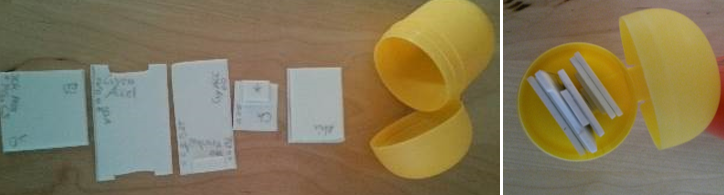
\includegraphics[width=1\textwidth]{images/k3-machbarkeitsstudie.PNG}
	\caption {Machbarkeitsstudie: Nachbau der Module mit Hilfe von Moosgummi}
	\label{fig:k3_machbarkeitsstudie}
\end{figure}

Die Wiring-Skizze in Abbildung \ref{fig:k3_wiringskizze} zeigt die Verbindungen der einzelnen Module untereinander. Diese ist nicht maßstabsgetreu. Ziel war es, alle Module korrekt miteinander verbinden zu können. Damit konnten auch schon erste Überlegungen angestellt werden, wie die Module später auch in der Kapsel angeordnet werden könnten. Letztendlich wird die Skizze auch hilfreich beim Löten sein.

\begin{figure}[h]
	\centering
	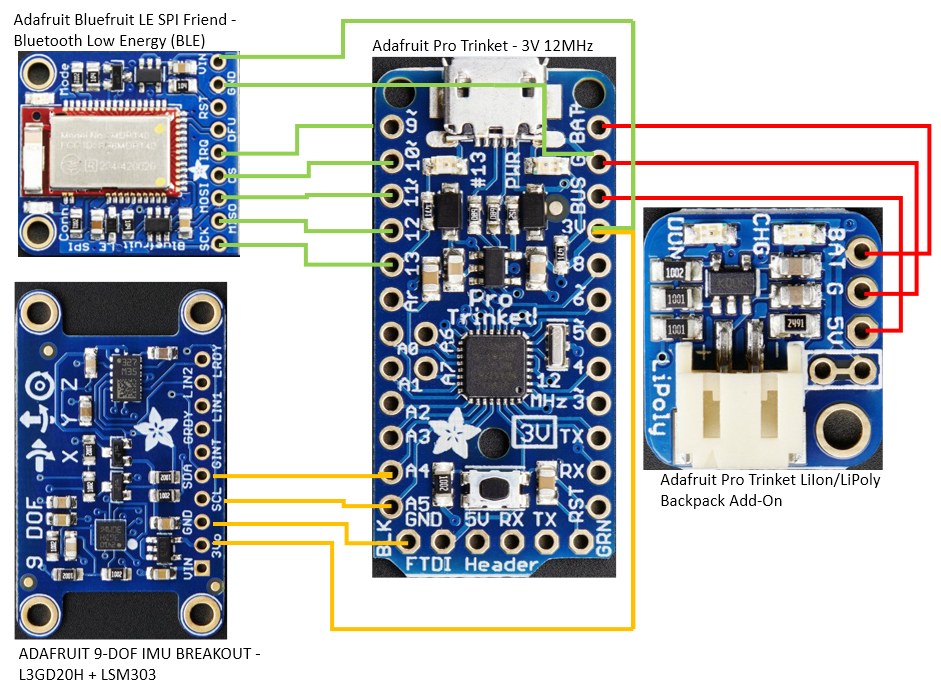
\includegraphics[width=0.9\textwidth]{images/k3-wiringskizze.PNG}
	\caption {Wiring-Skizze, wie die Bauteile miteinander verbunden werden}
	\label{fig:k3_wiringskizze}
\end{figure}

Nach positiven Ergebnissen aus den Machbarkeitsstudien wurden die Bauteile wie sie in Tabelle \ref{tab:bestellteHW} aufgeführt sind, bestellt. Da die Bestellung bei einem Händler getätigt wurde, waren die Bauteile in der folgenden Woche schon verfügbar.
\newpage

\subsubsection{Prototyping}

Für einen ersten Prototyp wurden die Bauteile mit Hilfe eines Breadboards und Steckkabeln miteinander verbunden. Zuerst wurden die Pro Trinkets getestet. (Hier ist leider ein Defekt eines Pro Trinkets aufgefallen.) Anschließend wurde das Bluetooth-Modul und zum Schluss das Sensor-Modul hinzugenommen.

\begin{figure}[h]
	\centering
	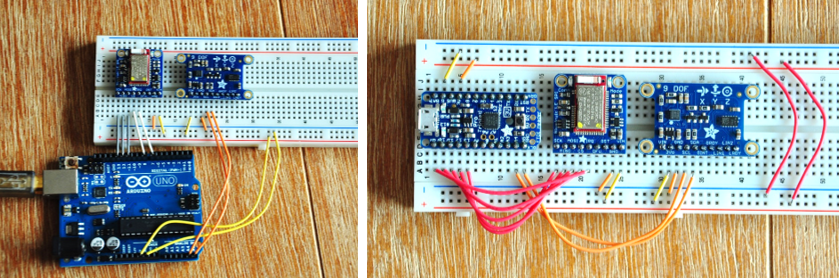
\includegraphics[width=1\textwidth]{images/k3-prototyping.PNG}
	\caption {Links: Prototyping mit dem Arduino Uno; Rechts: Prototyping mit dem Adafruit Pro
		Trinket}
	\label{fig:k3_prototyping}
\end{figure}

An dieser Stelle wurde außer dem Adafruit Pro Trinket noch ein Arduino Uno hinzugenommen, um während der Programmierung des Mikrocontrollers (siehe Kapitel \ref{kapitel_programmierungMikrocontroller}) auch mit einer Seriellen Ausgabe testen zu können. Bei erfolgreichem Testen des Programmcodes wurde dieser dann auf den Adafruit Pro Trinket übertragen.
%Erwähnen warum Uno schon vorher?

\subsubsection{Löten}

Da drei Bausätze vorhanden waren, und nur einer für das Prototyping genutzt wurde, konnte mit dem Löten des ersten Bausatzes begonnen werden, der in die Ü-Ei Kapsel passen soll.
Abbildung \ref{fig:k3_erstesBauteilGeloetet} zeigt das fertig gelötete Bauteil.

\begin{figure}[ht]
	\centering
	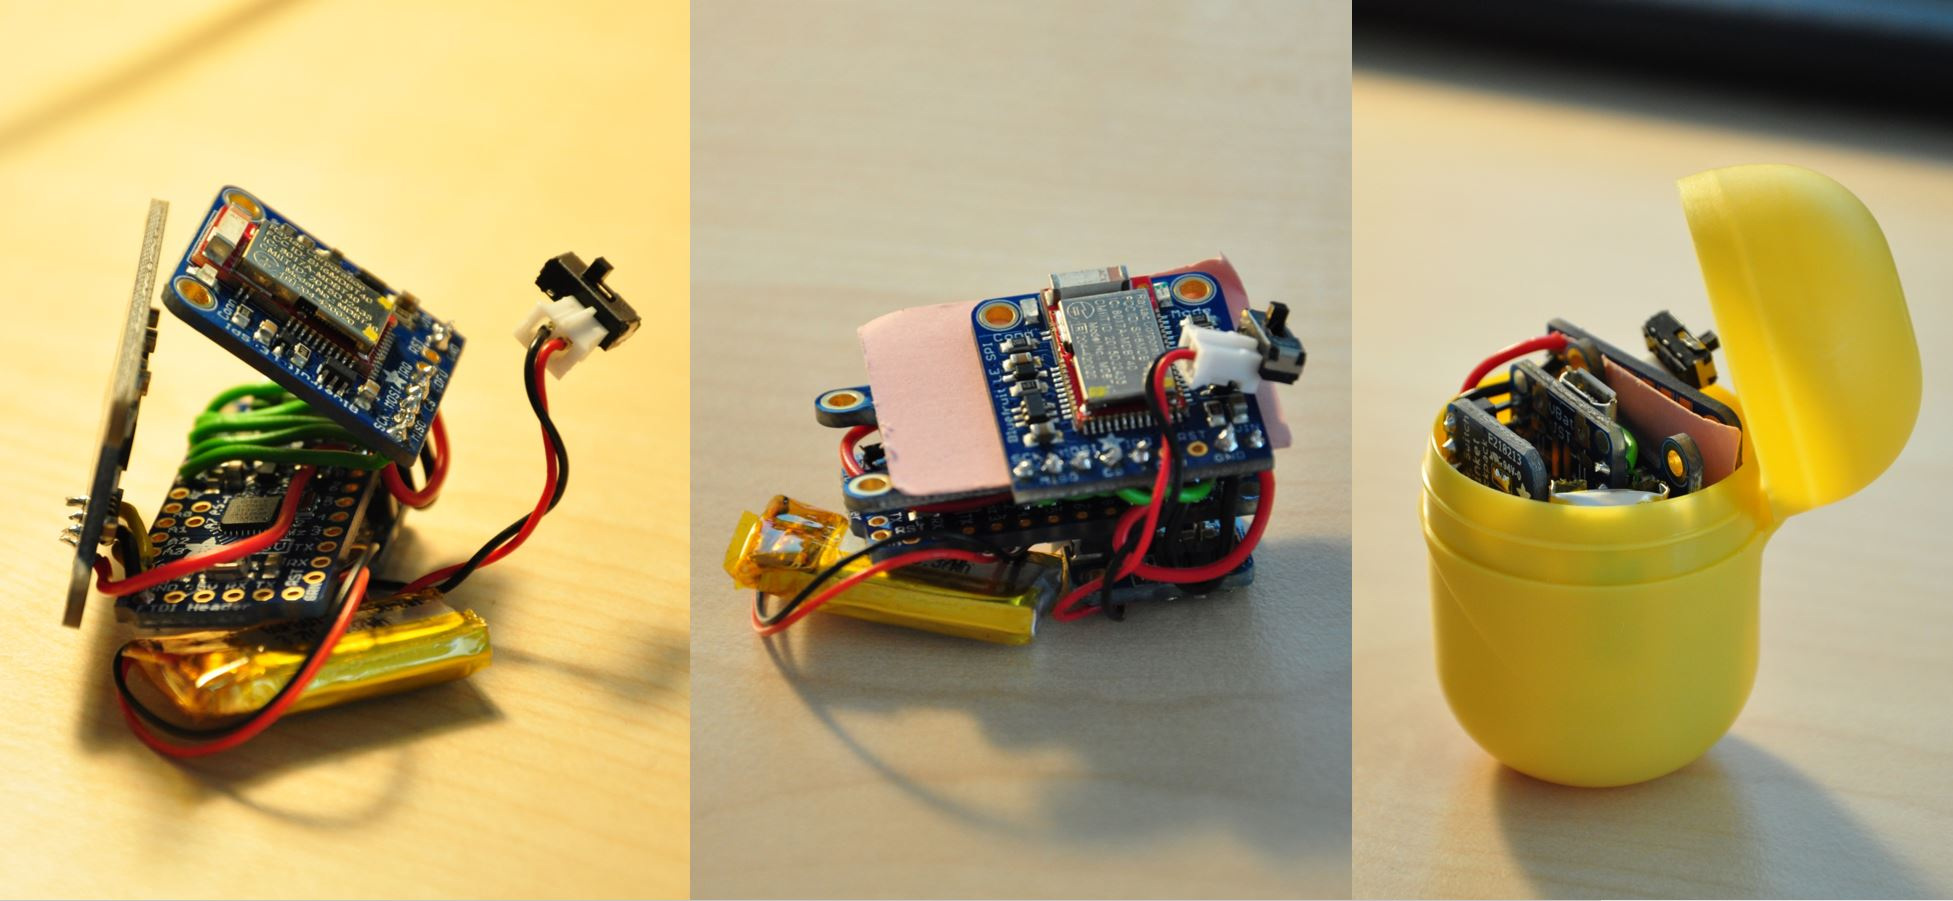
\includegraphics[width=1\textwidth]{images/k3-erstesBauteilGeloetet.jpg}
	\caption {Links: das erste gelötete Bauteil; Mitte: zwischen dem Bluetooth- und dem Sensor-
		Modul wird Papier zur Isolierung verwendet; Rechts: das Bauteil passt in eine Ü-Ei-Kapsel}
	\label{fig:k3_erstesBauteilGeloetet}
\end{figure}